\documentclass[a4paper,12pt]{article}
\usepackage[final]{graphicx}
\usepackage[utf8]{inputenc}
\usepackage[spanish]{babel}
\usepackage{amsmath}
\usepackage{listings}
\usepackage{xcolor}
\usepackage{hyperref}
\usepackage{geometry}
\usepackage{tocbibind}
\usepackage{float}
\usepackage[T1]{fontenc}
\usepackage[spanish]{babel}
\usepackage{tocloft}
\usepackage{caption}
\usepackage{subcaption}


\title{
    \vspace{4cm} % Ajusta este valor para centrar verticalmente
    \textbf{\Huge Memoria del Proyecto: \\ Aplicación de Machine Learning en Ajedrez} % Título en grande y negrita
}
\author{\Large Autor: Jesús González Suárez} % Autor en tamaño más grande
\date{\today} % Fecha actual

\lstset{
    language=Python,
    basicstyle=\ttfamily\footnotesize,
    keywordstyle=\color{blue}\bfseries,
    stringstyle=\color{red},
    commentstyle=\color{green},
    frame=single,
    breaklines=true,
    numbers=left,
    numberstyle=\tiny,
    xleftmargin=2em,
    framexleftmargin=1.5em
}

\begin{document}

\maketitle
\newpage

\tableofcontents
\newpage
\listoffigures
\newpage

\section{Introducción}

El presente proyecto tiene como objetivo explorar la integración de técnicas de \textit{Machine Learning} (ML) en el análisis del ajedrez. Se desarrollaron modelos capaces de:
\begin{itemize}
    \item Sugerir movimientos en base a una posición del tablero.
    \item Predecir resultados de partidas (ganador y duración).
    \item Analizar patrones de juego mediante técnicas de agrupamiento (\textit{clustering}).
\end{itemize}

El proyecto se fundamenta en el uso de bibliotecas modernas de Python como \texttt{TensorFlow}, \texttt{scikit-learn}, y \texttt{pandas}. A continuación, se describe el flujo de trabajo, los métodos implementados y los resultados obtenidos.

\section{Metodología}

El proyecto se divide en las siguientes etapas:
\begin{enumerate}
    \item Preprocesamiento de datos y tokenización de movimientos.
    \item Entrenamiento de modelos supervisados y no supervisados.
    \item Desarrollo de una interfaz gráfica para sugerencia de movimientos.
    \item Evaluación y visualización de resultados.
\end{enumerate}

\subsection{Datos Utilizados}

Los datos provienen de un conjunto de partidas en formato PGN, almacenados en el archivo \texttt{games.csv}. Las características principales extraídas incluyen:
\begin{itemize}
    \item Número de turnos (\texttt{turns}).
    \item Ventaja de rating entre jugadores (\texttt{rating\_advantage\_white}).
    \item Duración de la partida en minutos (\texttt{game\_duration}).
    \item Jugador ganador (\texttt{winner}).
\end{itemize}

\subsection{Modelos Implementados}

Los siguientes modelos fueron utilizados en distintas tareas del proyecto:
\begin{itemize}
    \item \textbf{Sugerencia de movimientos:} Una red neuronal entrenada con \texttt{TensorFlow} para predecir el próximo movimiento basado en una secuencia previa.
    \item \textbf{Predicción de duración de la partida:} Modelos de regresión como \texttt{RandomForestRegressor}.
    \item \textbf{Predicción de ganador:} Clasificadores como \texttt{GradientBoostingClassifier} y \texttt{RandomForestClassifier}.
    \item \textbf{Clustering de patrones de juego:} Algoritmo \texttt{KMeans}.
\end{itemize}

\section{Desarrollo}

\subsection{Tokenización y Sugerencia de Movimientos}

El primer paso fue preparar un tokenizador para representar movimientos en un formato que pueda ser procesado por el modelo. A continuación se muestra el código usado:

\begin{lstlisting}[language=Python]
def prepare_and_save_tokenizer(moves, save_path):
    tokenizer = Tokenizer()
    tokenizer.fit_on_texts(moves)
    with open(save_path, 'wb') as f:
        joblib.dump(tokenizer, f)
    return tokenizer
\end{lstlisting}

El modelo utiliza una red neuronal para sugerir el siguiente movimiento, basada en secuencias de longitud máxima de 20 movimientos. La predicción se integra con un motor de ajedrez para verificar la validez del movimiento.

\newpage

\subsection{Predicción del Ganador y Duración de la Partida}

Para la predicción de resultados, se extrajeron características como el \texttt{rating} de ambos jugadores, la duración y el número de turnos. El pipeline incluye el uso de modelos supervisados. Un ejemplo de la evaluación de \texttt{RandomForestRegressor} para duración es:

\begin{lstlisting}[language=Python]
def predict_game_duration(X, y):
    X_train, X_test, y_train, y_test = train_test_split(X, y, test_size=0.3, random_state=42)
    model = RandomForestRegressor(random_state=42)
    model.fit(X_train, y_train)
    y_pred = model.predict(X_test)
    print(f"MAE: {mean_absolute_error(y_test, y_pred):.2f}")
    print(f"RMSE: {mean_squared_error(y_test, y_pred, squared=False):.2f}")
    return model
\end{lstlisting}

\subsection{Clustering}

El análisis no supervisado se realizó con \texttt{KMeans}, identificando clusters de partidas según las características de los jugadores (\texttt{rating} blanco y negro). Este enfoque ayuda a identificar patrones de juego comunes.

\begin{lstlisting}[language=Python]
def evaluate_clustering(data, n_clusters=3):
    scaler = StandardScaler()
    scaled_data = scaler.fit_transform(data)
    kmeans = KMeans(n_clusters=n_clusters, random_state=42)
    kmeans.fit(scaled_data)
    data['Cluster'] = kmeans.labels_
    return kmeans, data
\end{lstlisting}

\newpage
\subsection{Interfaz Gráfica}

Se desarrolló una interfaz gráfica en \texttt{Tkinter} que muestra el tablero de ajedrez y sugiere movimientos. La integración con la biblioteca \texttt{chess.svg} permite visualizar el tablero de manera interactiva.

\vspace{10pt} % Reduce el espacio vertical
\begin{figure}[H]
    \centering
    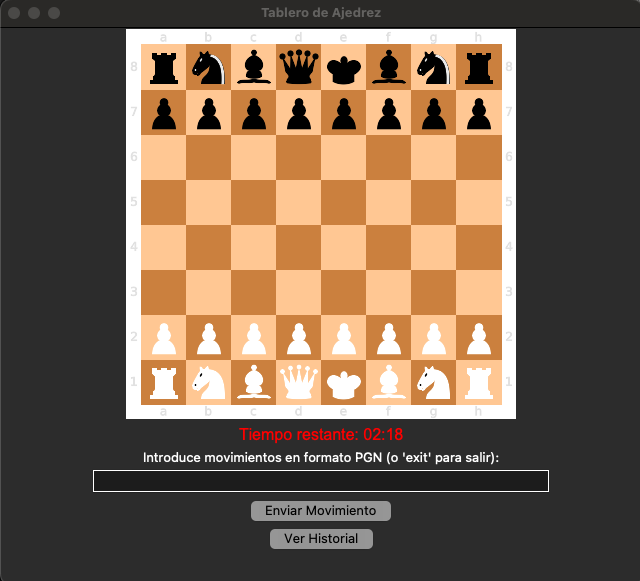
\includegraphics[width=\textwidth]{../images/Interfaz.png}
    \caption{Interfaz Modulo Ajedrez}
    \label{fig:Interfaz_Modulo_Ajedrez}
\end{figure}


\newpage
\section{Resultados}

\subsection{Sugerencia de Movimientos}

El modelo de red neuronal logró una precisión del 6\% en movimientos sugeridos en el conjunto de validación. La siguiente figura muestra la comparación entre movimientos sugeridos y reales:

\vspace{10pt} % Reduce el espacio vertical

\begin{figure}[H]
    \centering
    % Primera subfigura
    \begin{subfigure}[b]{\textwidth}
        \centering
        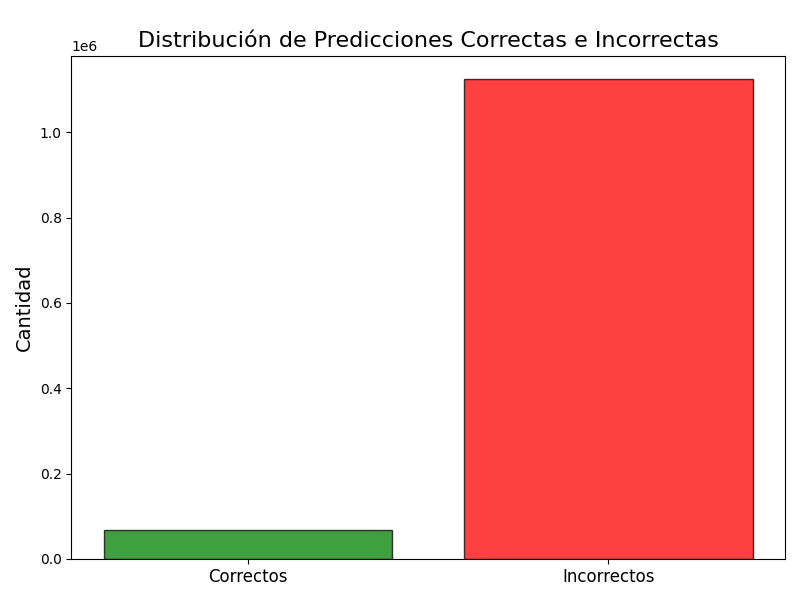
\includegraphics[width=0.6\textwidth]{../images/Figure_1_pred.png}
        \caption{Distribución Predicciones Correctas e Incorrectas}
        \label{fig:rDistribucion_Predicciones}
    \end{subfigure}
    
    \vspace{5pt} % Ajustar espacio entre las subfiguras
    
    % Segunda subfigura
    \begin{subfigure}[b]{\textwidth}
        \centering
        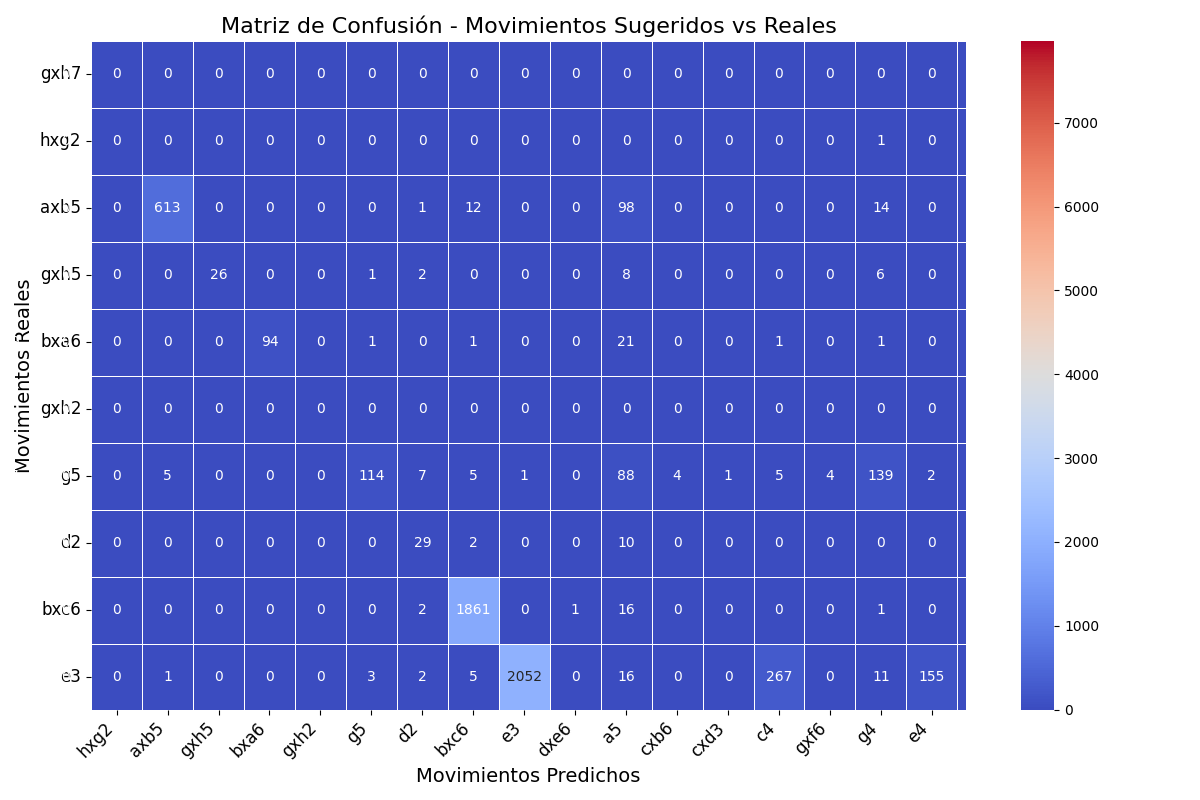
\includegraphics[width=0.6\textwidth]{../images/Figure_sug.png}
        \caption{Ejemplo Matriz de Confusión}
        \label{fig:Matriz_confusion}
    \end{subfigure}

    \caption{Comparación de Predicciones y Matriz de Confusión.}
    \label{fig:figuras_combinadas}
\end{figure}

\newpage

\subsection{Predicción de Ganador}

El modelo de \texttt{GradientBoostingClassifier} obtuvo una precisión promedio del 84\%. Para entrenar este modelo, se utilizaron las siguientes \textit{features} extraídas del conjunto de datos:

\begin{itemize}
    \item \textbf{Número de turnos:} Representa la cantidad total de movimientos realizados en la partida.
    \item \textbf{Puntuación del jugador blanco (\texttt{white\_rating}):} Valoración del jugador blanco al momento de jugar la partida.
    \item \textbf{Puntuación del jugador negro (\texttt{black\_rating}):} Valoración del jugador negro al momento de jugar la partida.
    \item \textbf{Ventaja de puntuación blanca:} Diferencia entre la puntuación del jugador blanco y la del jugador negro (\texttt{white\_rating - black\_rating}).
    \item \textbf{Duración de la partida:} Tiempo total que tomó la partida, medido en minutos.
    \item \textbf{Apertura (\texttt{opening\_ply}):} Número de movimientos realizados en la fase inicial de la partida.
\end{itemize}

La matriz de confusión presentada a continuación ilustra la comparación entre las etiquetas reales y las predicciones del modelo:

\vspace{10pt} % Reduce el espacio vertical
\begin{figure}[H]
    \centering
    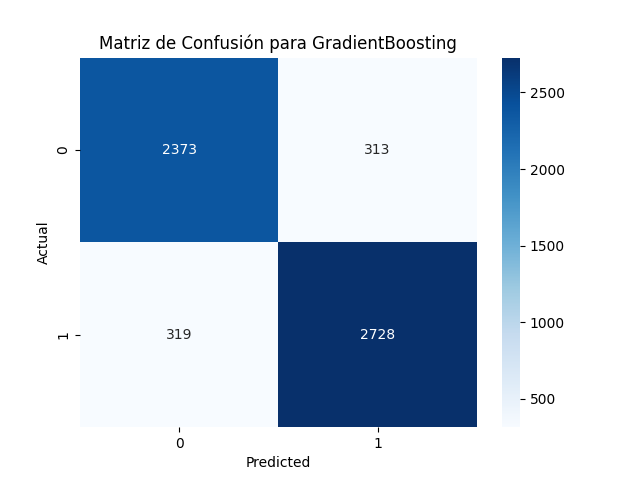
\includegraphics[width=0.7\textwidth]{../images/Figure_1_GB.png}
    \caption{Matriz de Confusión GradientBoostingClassifier}
    \label{fig:GradientBoostingClassifier}
\end{figure}

\subsection{Predicción de Duración de Partidas}

El objetivo de esta tarea fue construir un modelo capaz de predecir la duración de las partidas en minutos. Los datos utilizados incluyen características como:
\begin{itemize}
    \item \textbf{Diferencia de puntuaciones:} Diferencia entre las puntuaciones de los jugadores al inicio de la partida.
    \item \textbf{Número de turnos:} Total de movimientos realizados durante la partida.
    \item \textbf{Duración previa:} Basada en partidas similares en términos de apertura y estilo de juego.
\end{itemize}

Para este propósito, se utilizó un \texttt{RandomForestRegressor} con los siguientes hiperparámetros optimizados:
\begin{itemize}
    \item \textbf{n\_estimators:} 200
    \item \textbf{max\_depth:} 10
    \item \textbf{min\_samples\_leaf:} 2
\end{itemize}


El modelo alcanzó las siguientes métricas:
\begin{itemize}
    \item \textbf{Error absoluto medio (MAE):} 17.76 minutos.
    \item \textbf{Error cuadrático medio (RMSE):} 65.01 minutos.
\end{itemize}

La figura \ref{fig:duracion_partidas} muestra un gráfico de dispersión que compara las predicciones del modelo con los valores reales. La línea roja representa el ideal donde predicción y realidad coinciden perfectamente. 

\vspace{10pt} % Reduce el espacio vertical
\begin{figure}[H]
    \centering
    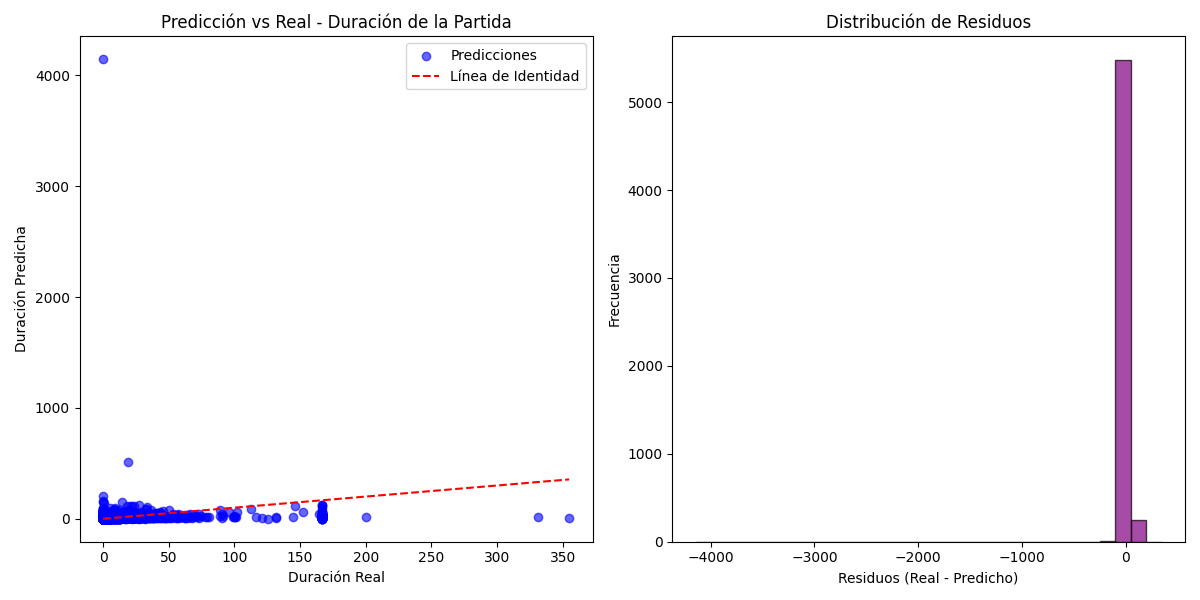
\includegraphics[width=0.8\textwidth]{../images/Figure_1_-dur_partidas.png}
    \caption{Predicción vs Real - Duración de Partidas}
    \label{fig:duracion_partidas}
\end{figure}

\textbf{Interpretación de Resultados:}
El modelo predice con un margen razonable de error en partidas de duración media, pero tiene dificultades con partidas extremadamente largas o cortas, lo que se refleja en el RMSE significativamente mayor al MAE. Esto sugiere que el modelo podría beneficiarse de:
\begin{itemize}
    \item Tratamiento de outliers en las partidas con duración extrema.
    \item Inclusión de características adicionales relacionadas con la estrategia de apertura.
\end{itemize}

\newpage

\subsection{Análisis de Clustering}

El análisis de clustering fue realizado para identificar patrones subyacentes en las partidas de ajedrez que no son evidentes a simple vista. Usamos el algoritmo de \textit{K-Means} para agrupar las partidas en función de características clave, como las puntuaciones de los jugadores y la duración de las partidas. El objetivo era descubrir grupos naturales de partidas basados en similitudes en las estadísticas del juego.

\textbf{Características utilizadas:}
\begin{itemize}
    \item \textbf{Puntuación del jugador blanco (\texttt{white\_rating}):} Representa la habilidad del jugador blanco según el sistema de puntuación del ajedrez.
    \item \textbf{Puntuación del jugador negro (\texttt{black\_rating}):} Similar al anterior, pero para el jugador negro.
    \item \textbf{Duración de la partida:} Tiempo total que tomó cada partida.
    \item \textbf{Número de turnos:} La cantidad de movimientos realizados en cada partida.
\end{itemize}

Estas características fueron seleccionadas porque proporcionan una visión integral del nivel de los jugadores y la complejidad de las partidas.

\textbf{Resultados del clustering:} El análisis reveló \textbf{tres grupos principales de partidas}:
\begin{itemize}
    \item \textbf{Cluster 1:} Partidas rápidas con jugadores de puntuación baja a media, lo que sugiere juegos casuales o menos competitivos.
    \item \textbf{Cluster 2:} Partidas de duración intermedia con jugadores de puntuación media, representando una mezcla de partidas semicompetitivas.
    \item \textbf{Cluster 3:} Partidas largas con jugadores de puntuación alta, lo que indica juegos de alto nivel, posiblemente en torneos.
\end{itemize}

\newpage

\textbf{Interpretación:} La separación en tres clusters destaca cómo el nivel de los jugadores y la duración de las partidas influyen en los patrones de juego. Los jugadores de mayor nivel tienden a tener partidas más largas, ya que analizan más profundamente sus movimientos, mientras que los jugadores casuales suelen jugar partidas más rápidas y menos estratégicas.

El siguiente gráfico ilustra esta clasificación, mostrando cómo los grupos se distribuyen en función de las puntuaciones de los jugadores y otras características clave:

\begin{figure}[H]
    \centering
    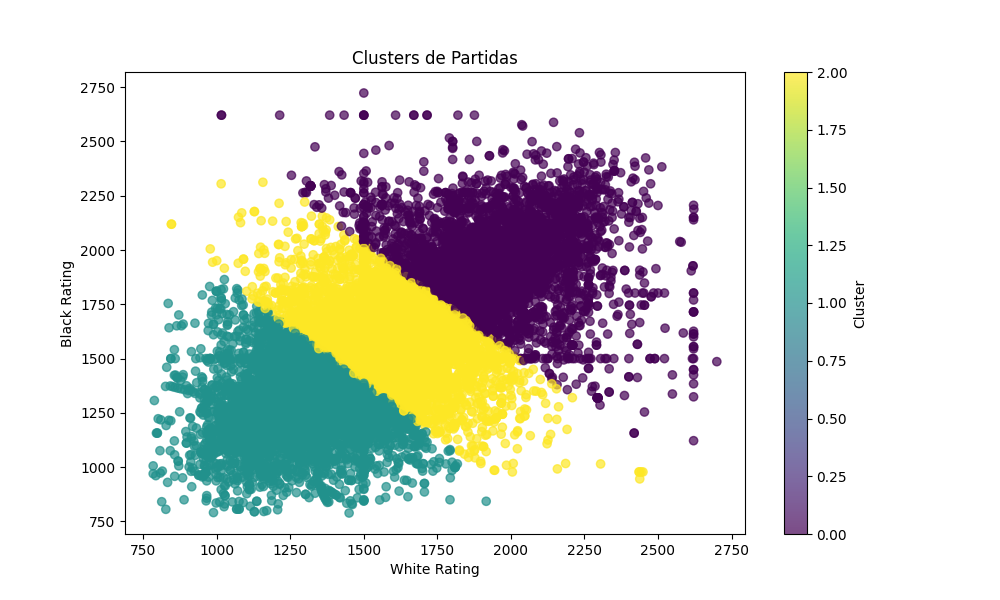
\includegraphics[width=0.8\textwidth]{../images/Figure_1_clustersPartidas.png}
    \caption{Clasificación de partidas mediante clustering.}
    \label{fig:clustering}
\end{figure}

\newpage

\section{Conclusión}

Este proyecto demuestra el potencial de aplicar \textit{Machine Learning} en el análisis del ajedrez. Las áreas principales de mejora incluyen:
\begin{itemize}
    \item Entrenar el modelo de sugerencia con conjuntos de datos más amplios.
    \item Explorar arquitecturas avanzadas como \textit{transformers}.
    \item Refinar las métricas para análisis de patrones.
\end{itemize}

\section*{Referencias}

\begin{itemize}
    \item \href{https://tensorflow.org}{TensorFlow Documentation}
    \item \href{https://scikit-learn.org}{Scikit-learn Documentation}
    \item \href{https://www.chess.com}{Chess.com Data API}
\end{itemize}

\end{document}
